\documentclass{article}
\usepackage[utf8]{inputenc}
\usepackage{graphicx}
\usepackage{subfigure}
\usepackage{subcaption}
\usepackage{wrapfig}


\author{Valère Preney}
\date{December 2020}
\title{Report Java Project - Mystic Tarot}

\begin{document}
\maketitle
\section{Introduction}\label{introduction}

Before begin any typing, I've made some research in order to know more about this ``practice''. And I've found all of what I needed here : https://www.apprendre-tarotdemarseille.com/ (All the images I used for the card are from this website by the way). The I've decided to start with Arcanes Mineures and Arcanes Majeures. And as I thought two classes
were not enought for basis of the project, I added one own-maded class. Arcanes Majestueuse is it.(More details in this report below - Classes Section) In a first hand I wrote all the classes that doesn't belong to the view part. So are they Player class, Card(Abstract class), ArcanesMajeures, Arcanes Mineures, Arcanes Majestueuses. All of them extended from Card Class. And all the view part was coded in a one single page. As I thought it wasn't really clean and properly coded I've decided to start all the project over again. Then I've coded the project by using the MVC design pattern, and the Observer principle. And there is differents classes in the view part that represents differents components of the application (Also more details in the report below)

\section{UML Diagram}\label{uml-diagram}

See the Class Diagram png in RapportProjet directory

\section{How to use it}\label{how-to-use-it}

\subsection{Form Welcome Panel}\label{form-welcome-panel}

Once the user has started the program, he has got to fill a welcome
form. He must enter his name and choose betwin two choices of a two
radioButton couple. Then he press enter and go into in.

\begin{figure}[htbp]
\centering
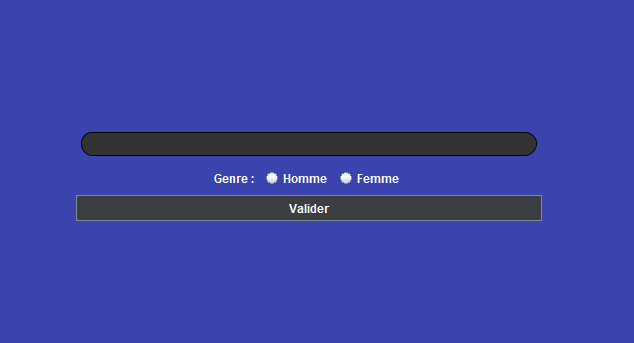
\includegraphics[width=10cm]{welcomeForm.PNG}
\caption{Form Welcom Panel}
\end{figure}

\subsection{Main Window}\label{main-window}

Then, once it's done, the user can see the program break down into
segments.

\begin{figure}[htbp]
\centering
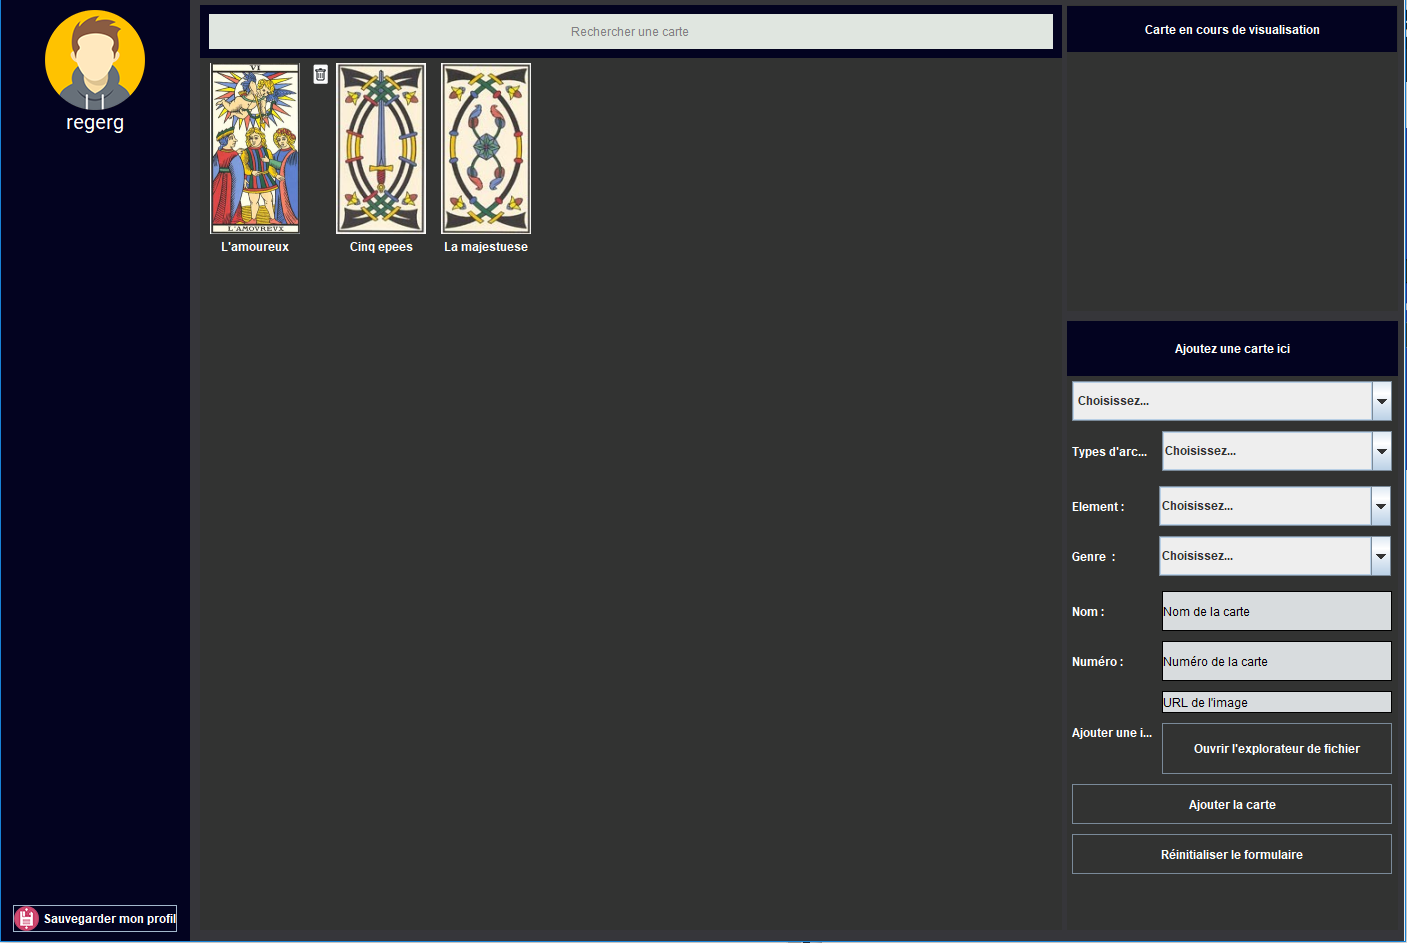
\includegraphics[width=10cm]{mainPage.png}
\caption{Main Page}
\end{figure}

\subsubsection{The SideBar}\label{a---the-sidebar}

First you've got the side bar with a little icon, the name and at save profil button at the bottom.
\begin{figure}[htbp]
    \centering
    \begin{minipage}{.3\textwidth}
        \centering
        
\includegraphics{avatar.png}
        \caption{Male Icon}
    \end{minipage}%
    \begin{minipage}{.3\textwidth}
        \centering
         
\includegraphics{avatar2.png}
         \caption{Female Icon}
    \end{minipage}%
    \begin{minipage}{.3\textwidth}
        \centering
        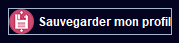
\includegraphics{saveBtn.PNG}
        \caption{save button}
    \end{minipage}
\end{figure}

            
           
 

\subsubsection{The central panel - collection card and search
bar}\label{the-central-panel---collection-card-and-search-bar}

Then you can see a central panel. Here released a search bar and the
card collection of the user. Each card will be set with a respective
image and a name.

\begin{figure}[htbp]
\centering
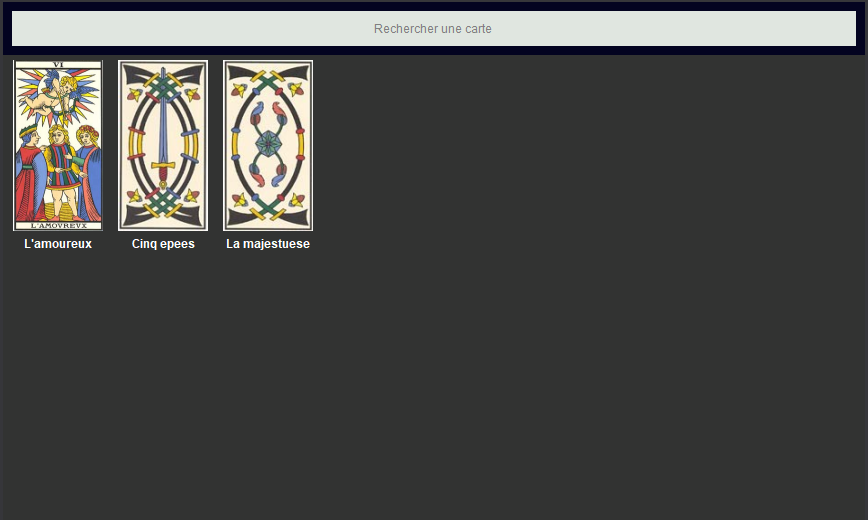
\includegraphics[width=10cm]{collectionCard.PNG}
\caption{Collection Card}
\end{figure}

By hovering one of these card, a dustbin icon will pop

\includegraphics{dustbinIcon.PNG}just on the left of the card
image so you can remove the card from you're collection.

\subsubsection{The detail Panel}\label{c---the-detail-panel}

By clicking on one of these card you set the top-right panel : detail
Panel. Here you will see the detail of the card you've just clicked on
before.

\begin{figure}[htbp]
    \centering
    \begin{minipage}{.5\textwidth}
        \centering
        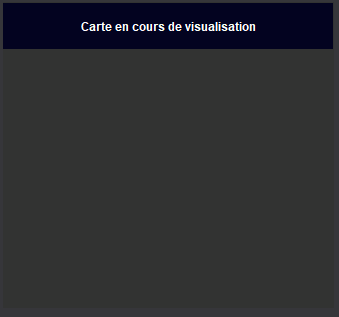
\includegraphics[scale=0.5]{detailEmpty.PNG}
        \caption{Empty Panel Detail}
    \end{minipage}%
    \begin{minipage}{.5\textwidth}
        \centering
         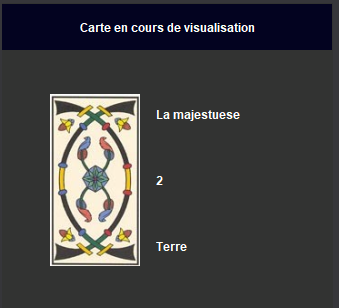
\includegraphics[scale=0.5]{detail.PNG}
         \caption{Panel Detail}
    \end{minipage}
\end{figure}

By hovering each property value on the right of the image, a pen icon will pop 
\includegraphics{edit.png} so you can set the property
that belong to the icon. JLabel will turn into JTextField or JComboBox. Depending on the nature of the property you're setting. To validate your change, where the edit icon was a validate icon

\includegraphics{valid.png} is instead.

\subsubsection{The adding form}\label{d---the-adding-form}
And finally the adding form there is. With this, you will can add new card to your collection.

\begin{block}
\begin{wrapfigure}{l}{0.4\textwidth}
    \begin{center}
        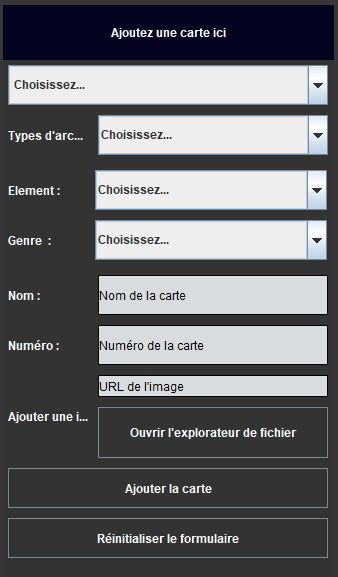
\includegraphics[scale=0.5]{formAdd.PNG}
    \end{center}
     \caption{Adding Form}
\end{wrapfigure}
There is different options :
\begin{enumerate}
\item You can add a card by choosing one of the default card. Once the choice done, the form will automatically be filled. Then you will be uncapable to modify the fields unless you clickon the empty form button.
\item Otherwise you can create your own card by choosing the item you want in the combobox components and typing the right word in the text fields components. But the first combobox, the default card proposal, must remained unchoosen. It means the first item (``choisissez une carte'') must be selected.
\end{enumerate}
\end{block}


\section{The Project Structure}\label{the-project-structure}
\subsection{The View - Package}\label{the-view---package}
This package contains all what's important for the user interface.
\subsubsection{The interfaces}\label{the-interfaces}
These interfaces are required when the user
trigger the event by using the linked component. To do so, I've been
thinking like that : there is one component that trigger the event and the event listener calls the corresponding method in the linked Panel which implements the needed interface. The bound between both component (component trigger, (interface)panel calling method) is created in a static HashMap set in the View Page. Most of the time the panel linked to the trigger component is the panel that contains the trigger component. But not for one time where the panel needed to be listen is send to the class that contains the trigger component. By doing like this you have juste two lines of code to write into the EventListener Classes. It doesn't matter which component add an event to his listener.
\begin{enumerate}
\item IGotBtnClickable
\item IGotBtnHover
\item IGotComboxChange
\item IGotFocusComponent
\item IGotTextFieldKeyListening
\end{enumerate}
\subsubsection{The Classes}\label{the-classes}
\begin{itemize}
 \item View Page
     \begin{itemize}
     \item FormPanelWelcome
        \begin{itemize}
             \item RoundedJTextField
             \item RoundedBorderCorner
        \end{itemize}
     \item PanelMainPage
        \begin{itemize}
             \item PanelSideBar
             \item PanelCollectionCard
                \begin{itemize}
                \item CardPanel
                \item CardIsJButton
                \end{itemize}
             \item PanelDetailCard
                \begin{itemize}
                \item AsbtractPanelForArcanesType
                \item PanelForArcanesMajestueuseDetail
                \item PanelForArcanesMajeureDetail
                \item PanelForArcanesMineureDetail
                \end{itemize}
             \item PanelFormAddCard
                \begin{itemize}
                \item ListRenderer
                \end{itemize}
        \end{itemize}
     \end{itemize}
 \item EventListenerClasses
    \begin{itemize}
    \item ButtonAction
    \item ComboBoxAction
    \item FocusAction
    \item KeyPressedAction
    \end{itemize}
\end{itemize}


\subsection{The Controller - Package}\label{the-controller---package}

This package is like a ferryman. Every change triggered in the view
package (by the user) will be set in the classes model package. \subsubsection{The classes}\label{the-classes}
\begin{enumerate}
    \item AbstractControllerPlayer
    \item ControllerPlayer
\end{enumerate}

\subsection{The Model - Package}\label{the-model---package}

\subsubsection{The Interfaces}\label{a---the-interfaces}
This interface takes care of the sustainability of the essentials data and as for it, Player is the only class to implements the interface.
\begin{enumerate}
    \item IsSustainable
\end{enumerate}

\subsubsection{ The Classes }\label{the-classes}
\begin{enumerate}
    \item AbstractModel
    \item Player
    \item Card
    \item ArcanesMajeures
    \item ArcanesMineures
    \item ArcanesMajestueuses
\end{enumerate} 

\subsection{The Observer - Package}\label{the-observer---package}

This package well carrying his name. Every oberved change in th model will reset the view. Once the change is set into the corresponding model class, the observable classes call the method
\texttt{notifyObserver(Player p)} that inform all the observers.
\subsubsection{The interface}\label{the-interfaces}
\begin{enumerate}
    \item Observable
    \item Observer
\end{enumerate}
\end{document}
